\documentclass[aspectratio=169,11pt]{beamer}

\usetheme{Madrid}
\usecolortheme{default}
\setbeamertemplate{navigation symbols}{}

\usepackage[T1]{fontenc}
\usepackage[utf8]{inputenc}
\usepackage{lmodern}
\usepackage{amsmath,amssymb}
\usepackage{booktabs}
\usepackage{tikz}
\usepackage{graphicx}
\usetikzlibrary{arrows.meta,positioning,shapes.geometric,fit}

\title[SAANS]{Symmetry-Safe Adaptive Noise Scheduling for\\E(3)-Equivariant Diffusion Training}
\subtitle{EECE 571F Project Presentation}
\author{Abdelrahman Ahmed}
\date{\today}

\definecolor{saansblue}{RGB}{27,79,114}
\definecolor{saansorange}{RGB}{211,84,0}
\definecolor{saansgreen}{RGB}{34,139,34}

\begin{document}

\begin{frame}
    \titlepage
\end{frame}

\begin{frame}{1. Motivation and Problem}
\footnotesize
\begin{columns}[T]
    \begin{column}{0.56\textwidth}
        \begin{itemize}
            \item Diffusion models train over many noise levels, but most implementations use a fixed timestep schedule.
            \item Different timestep regions can have very different difficulty, variance, and optimization value.
            \item In 3D molecular diffusion, this matters even more because the model must denoise while preserving \textbf{E(3) symmetry}.
        \end{itemize}

        \vspace{0.25em}
        \begin{block}{Core question}
        Can we spend more training effort on hard timestep regions \emph{without} changing the baseline objective?
        \end{block}

        \begin{alertblock}{Why this matters}
        If successful, we learn whether training compute can be allocated more efficiently in equivariant molecular diffusion.
        \end{alertblock}
    \end{column}
    \begin{column}{0.40\textwidth}
        \centering
        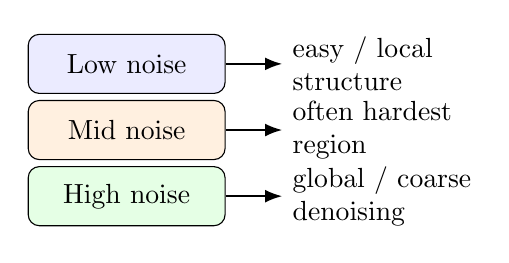
\begin{tikzpicture}[scale=0.8]
            \node[draw, rounded corners, fill=blue!8, minimum width=2.5cm, minimum height=0.75cm] (l) at (0,2.0) {Low noise};
            \node[draw, rounded corners, fill=orange!12, minimum width=2.5cm, minimum height=0.75cm] (m) at (0,0.95) {Mid noise};
            \node[draw, rounded corners, fill=green!10, minimum width=2.5cm, minimum height=0.75cm] (h) at (0,-0.1) {High noise};

            \draw[-{Latex[length=2.2mm]}, thick] (l.east) -- +(0.9,0) node[right, align=left] {easy / local\\structure};
            \draw[-{Latex[length=2.2mm]}, thick] (m.east) -- +(0.9,0) node[right, align=left] {often hardest\\region};
            \draw[-{Latex[length=2.2mm]}, thick] (h.east) -- +(0.9,0) node[right, align=left] {global / coarse\\denoising};
        \end{tikzpicture}
    \end{column}
\end{columns}
\end{frame}

\begin{frame}{2. Related Work and Project Gap}
\small
\begin{table}
\centering
\begin{tabular}{p{0.28\textwidth}p{0.60\textwidth}}
\toprule
\textbf{Area} & \textbf{Takeaway} \\
\midrule
Equivariant molecular diffusion & Strong baselines already exist for 3D molecule generation; we build on them instead of inventing a new backbone. \\
Diffusion scheduling / weighting & Prior work suggests timestep choice matters for optimization efficiency and variance. \\
Our project gap & Very little work studies \textbf{symmetry-safe adaptive timestep allocation} for \textbf{E(3)-equivariant} molecular diffusion. \\
\bottomrule
\end{tabular}
\end{table}

\vspace{0.3em}
\begin{block}{Our positioning}
This is a \textbf{training-time optimization project}, not a new molecule generator architecture.
\end{block}

\begin{itemize}
    \item Baseline: public EDM-style equivariant molecular diffusion codebase.
    \item Goal: improve how timesteps are sampled during training.
    \item Constraint: preserve the original objective in expectation and use symmetry-safe hardness signals.
\end{itemize}
\end{frame}

\begin{frame}{3. Main Idea: SAANS}
\footnotesize
\begin{columns}[T]
    \begin{column}{0.52\textwidth}
        \begin{itemize}
            \item Partition timesteps into bins $I_1,\dots,I_B$.
            \item Track a detached hardness estimate $S_b$ for each bin.
            \item Define an adaptive distribution:
            \[
            q_b \propto p_{0,b}(\varepsilon + S_b)^{\alpha}
            \]
            \item Mix with the baseline for stability and full support.
            \item Importance-weight each sampled bin by
            \[
            w_b = \frac{p_{0,b}}{q_b}
            \]
        \end{itemize}

        \begin{alertblock}{Key design constraint}
        Hardness estimates should be \textbf{symmetry-safe}: they should not change under arbitrary rotations or translations.
        \end{alertblock}
    \end{column}
    \begin{column}{0.44\textwidth}
        \centering
        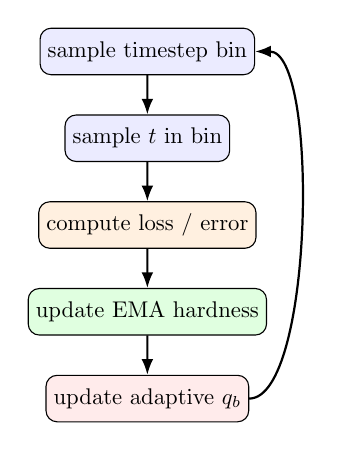
\begin{tikzpicture}[node distance=0.5cm, scale=0.82, every node/.style={scale=0.82}]
            \node[draw, rounded corners, fill=blue!8, minimum width=2.5cm, minimum height=0.72cm] (a) {sample timestep bin};
            \node[draw, rounded corners, fill=blue!8, below=of a, minimum width=2.5cm, minimum height=0.72cm] (b) {sample $t$ in bin};
            \node[draw, rounded corners, fill=orange!12, below=of b, minimum width=2.5cm, minimum height=0.72cm] (c) {compute loss / error};
            \node[draw, rounded corners, fill=green!12, below=of c, minimum width=2.5cm, minimum height=0.72cm] (d) {update EMA hardness};
            \node[draw, rounded corners, fill=red!8, below=of d, minimum width=2.5cm, minimum height=0.72cm] (e) {update adaptive $q_b$};

            \draw[-{Latex[length=2mm]}, thick] (a) -- (b);
            \draw[-{Latex[length=2mm]}, thick] (b) -- (c);
            \draw[-{Latex[length=2mm]}, thick] (c) -- (d);
            \draw[-{Latex[length=2mm]}, thick] (d) -- (e);
            \draw[-{Latex[length=2mm]}, thick] (e.east) .. controls +(1.0,0) and +(1.0,0) .. (a.east);
        \end{tikzpicture}
    \end{column}
\end{columns}
\end{frame}

\begin{frame}{4. Draft Main Figure: Reallocating Timestep Mass}
\small
\begin{center}
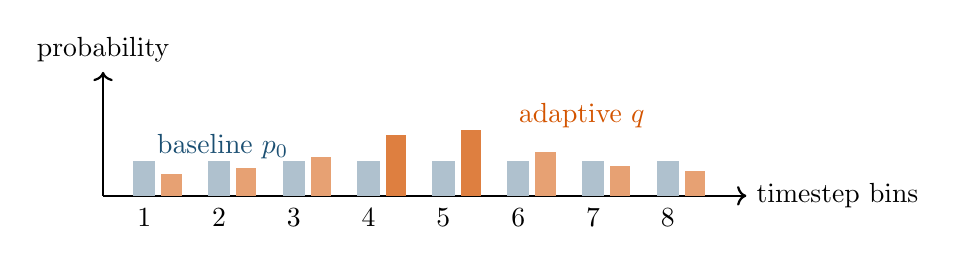
\begin{tikzpicture}[x=0.95cm,y=3.5cm]
    % axes
    \draw[->, thick] (0,0) -- (8.6,0) node[right] {timestep bins};
    \draw[->, thick] (0,0) -- (0,0.45) node[above] {probability};

    % baseline bars
    \foreach \x in {0,...,7} {
        \fill[saansblue!35] (0.4+\x,0) rectangle (0.7+\x,0.125);
    }
    \node[saansblue] at (1.6,0.18) {baseline $p_0$};

    % adaptive bars
    \fill[saansorange!55] (0.78,0) rectangle (1.05,0.08);
    \fill[saansorange!55] (1.78,0) rectangle (2.05,0.10);
    \fill[saansorange!55] (2.78,0) rectangle (3.05,0.14);
    \fill[saansorange!75] (3.78,0) rectangle (4.05,0.22);
    \fill[saansorange!75] (4.78,0) rectangle (5.05,0.24);
    \fill[saansorange!55] (5.78,0) rectangle (6.05,0.16);
    \fill[saansorange!55] (6.78,0) rectangle (7.05,0.11);
    \fill[saansorange!55] (7.78,0) rectangle (8.05,0.09);
    \node[saansorange] at (6.4,0.29) {adaptive $q$};

    % bin labels
    \foreach \x/\lab in {0.55/1,1.55/2,2.55/3,3.55/4,4.55/5,5.55/6,6.55/7,7.55/8} {
        \node[below] at (\x,-0.01) {\lab};
    }
\end{tikzpicture}
\end{center}

\begin{block}{Interpretation}
Illustrative draft figure: the baseline schedule is fixed, while SAANS shifts probability mass toward bins that appear harder under training diagnostics.
\end{block}

\begin{itemize}
    \item Final paper figure should show how $q_b$ evolves over training.
    \item We also want matching plots for hardness EMA, occupancy, and per-bin loss variance.
\end{itemize}
\end{frame}

\begin{frame}{5. Planned Experiments and Current Status}
\small
\begin{columns}[T]
    \begin{column}{0.54\textwidth}
        \begin{block}{Planned QM9 study}
        \begin{itemize}
            \item Baseline EDM scheduler
            \item Full SAANS
            \item Adaptive without importance weighting
            \item Hardness variants and scheduler sweeps
        \end{itemize}
        \end{block}

        \begin{block}{What we want to learn}
        \begin{itemize}
            \item Which timestep regions are hardest?
            \item Does adaptive allocation improve optimization efficiency?
            \item Is importance weighting necessary?
            \item Does symmetry-safe hardness matter?
        \end{itemize}
        \end{block}
    \end{column}
    \begin{column}{0.42\textwidth}
        \begin{block}{Current project status}
        \begin{itemize}
            \item Public EDM baseline integrated
            \item QM9 pipeline working locally
            \item Smoke tests for baseline and SAANS completed
            \item Short-run comparison pipeline built
        \end{itemize}
        \end{block}

        \begin{alertblock}{Important caveat}
        Current numbers are only \textbf{smoke-test engineering checks}, not publication-grade results.
        \end{alertblock}
    \end{column}
\end{columns}
\end{frame}

\begin{frame}{6. Takeaway}
\small
\begin{itemize}
    \item We study \textbf{adaptive timestep allocation} for \textbf{E(3)-equivariant molecular diffusion}.
    \item The project contributes a \textbf{training-time scheduler} rather than a new backbone.
    \item The key idea is to reallocate probability mass toward hard timestep regions while preserving the baseline objective through importance weighting.
    \item The implementation scaffold, baseline integration, QM9 pipeline, diagnostics, and short-run SAANS tests are already in place.
    \item The next step is to run longer GPU experiments and evaluate whether SAANS improves efficiency and generation quality.
\end{itemize}

\vspace{0.5em}
\centering
\Large Questions?
\end{frame}

\end{document}